\documentclass[a0paper,landscape]{a0poster}
\usepackage[utf8]{inputenc}
\usepackage[spanish]{babel}
\usepackage{lmodern} % Fuentes escalables
\usepackage{graphicx}
\usepackage{xcolor}
\usepackage{multicol}
\usepackage{array}
\usepackage{geometry}
\usepackage{booktabs}
\usepackage{amssymb}
\usepackage{tikz}
\usepackage{environ}
\usetikzlibrary{shapes,arrows,positioning,shadows,trees,fit,backgrounds,babel}

% Configurar márgenes optimizados para A0 landscape
\geometry{margin=1.5cm, top=0.5cm, bottom=1.0cm}
\setlength{\parindent}{0pt}
\setlength{\parskip}{0.06cm}

% Paleta de colores UC (Pontificia Universidad Católica)
\definecolor{ucred}{RGB}{200, 16, 46}          % Rojo UC oficial
\definecolor{ucblue}{RGB}{0, 56, 147}          % Azul UC oficial
\definecolor{uclight}{RGB}{244, 245, 247}      % Gris claro UC
\definecolor{ucgreen}{RGB}{34, 139, 34}        % Verde para soluciones
\definecolor{darktext}{RGB}{33, 37, 41}        % Texto oscuro UC

% ============================================================
% DEFINICIÓN DE CAJA ESTILO PÓSTER (SECTIONBOX)
% ============================================================
\newsavebox{\sectionboxcontent}
\NewEnviron{sectionbox}[2]{% #1=Color, #2=Title
\savebox{\sectionboxcontent}{%
    \begin{minipage}{0.95\linewidth}
        \vspace{20pt}
        \BODY
        \vspace{6pt}
    \end{minipage}%
}
\begin{center}
\begin{tikzpicture}
\node [
    draw=#1,
    line width=2pt,
    fill=white,
    rounded corners=15pt,
    drop shadow={opacity=0.3,shadow xshift=3pt,shadow yshift=-3pt},
    inner sep=10pt
] (box) {
    \usebox{\sectionboxcontent}
};
\node[
    fill=#1,
    text=white,
    font=\bfseries\LARGE,
    rounded corners=10pt,
    anchor=west,
    xshift=20pt
] at (box.north west) { \vphantom{Ag} #2 };
\end{tikzpicture}
\end{center}
\vspace{0.3cm}
}

\begin{document}
\shorthandoff{>}\shorthandoff{<}

% ============================================================
% ENCABEZADO PROFESIONAL CON LOGOS
% ============================================================
\begin{center}

% Logos en minipage
\begin{minipage}[t]{0.15\textwidth}
\centering

\includegraphics[width=0.95\textwidth]{../../Logos/logo-uc-02.pdf}
\end{minipage}%
\hfill
\begin{minipage}[t]{0.73\textwidth}
\centering
\vspace{-7.5cm}

% TÍTULO PRINCIPAL - MÁS GRANDE
{\fontsize{135}{150}\selectfont \textcolor{ucblue}{\textbf{ALGORITMOS Y POLARIZACIÓN POLÍTICA}}}

\vspace{0.2cm}

% Subtítulo
{\fontsize{75}{85}\selectfont \textcolor{ucblue}{\textbf{Panorámica de la Democracia Chilena 2021-2025}}}

\vspace{0.2cm}

% Información institucional
{\fontsize{35}{40}\selectfont \textcolor{darktext}{Proyecto Final — Ética de la IA — Pontificia Universidad Católica}}

\vspace{-0.2cm}
\end{minipage}%

\vspace{0.1cm}

% Línea decorativa profesional
\noindent\makebox[\linewidth]{\textcolor{ucblue}{\rule{\textwidth}{6pt}}}

\vspace{0.2cm}

\end{center}

% ============================================================
% CONTENIDO EN 3 COLUMNAS CON MEJOR ESTRUCTURA
% ============================================================
\setlength{\columnsep}{0.6cm}
\setlength{\columnseprule}{1.5pt}
\def\columnseprulecolor{\color{ucblue}}

\begin{multicols}{3}

% ============================================================
% COLUMNA 1
% ============================================================

\begin{sectionbox}{ucred}{POSTURA CENTRAL}

\fcolorbox{ucred}{uclight}{%
\begin{minipage}[c]{0.96\linewidth}
{\fontsize{22}{26}\selectfont \textbf{\textcolor{darktext}{``Si bien los algoritmos de redes sociales facilitan la polarización, el factor determinante en la erosión democrática en Chile no es la tecnología per se, sino la ausencia de un marco regulatorio efectivo que sancione su instrumentalización deliberada por actores políticos para difundir desinformación coordinada.''}}}
\end{minipage}%
}

\vspace{0.2cm}

\subsection*{\textcolor{ucblue}{\Large Tres Consecuencias Negativas}}
{\fontsize{20}{24}\selectfont
\begin{itemize}
    \setlength{\itemsep}{0.15cm}
    \item[\textcolor{ucred}{\textbf{\ensuremath{\blacktriangleright}}}] \textbf{Limitación del diálogo}: ``Burbujas de filtro'' impiden exposición diversa
    \item[\textcolor{ucred}{\textbf{\ensuremath{\blacktriangleright}}}] \textbf{Facilitación de desinformación}: Algoritmos priorizan engagement
    \item[\textcolor{ucred}{\textbf{\ensuremath{\blacktriangleright}}}] \textbf{Reproducción de sesgos}: IA aprende y refuerza prejuicios
\end{itemize}
}

\vspace{0.2cm}
\fcolorbox{ucblue}{white}{%
\begin{minipage}[c]{0.96\linewidth}
\centering
{\fontsize{20}{24}\selectfont \textit{``La desinformación es un problema tecnológico en su forma, pero profundamente humano en su fondo.''}}
\end{minipage}%
}

\vspace{0.3cm}

\begin{center}
\begin{tikzpicture}[>=stealth, thick, scale=0.9, transform shape]
    % Nodos con tamaño fijo y ancho de texto ajustado para evitar desbordes
    \node[draw, circle, fill=uclight, minimum size=6cm, text width=5.2cm, align=center, drop shadow, font=\fontsize{16}{19}\selectfont] (pol) at (0, 3.5) {\textbf{POLARIZACIÓN}};
    
    \node[draw, circle, fill=uclight, minimum size=6cm, text width=5.2cm, align=center, drop shadow, font=\fontsize{16}{19}\selectfont] (des) at (6, -3.5) {\textbf{DESINFORMACIÓN}};
    
    \node[draw, circle, fill=ucred, text=white, minimum size=6cm, text width=5.2cm, align=center, drop shadow, font=\fontsize{16}{19}\selectfont] (mas) at (-6, -3.5) {\textbf{MÁS POLARIZACIÓN}};

    % Flechas con curvatura ajustada
    \draw[->, ucred, line width=3.5pt] (pol) to[bend left=25] (des);
    \draw[->, ucred, line width=3.5pt] (des) to[bend left=25] (mas);
    \draw[->, ucred, line width=3.5pt] (mas) to[bend left=25] (pol);

    % Fuente
    \node[below=0.5cm, font=\small\itshape, text=gray] at (0,-7) {Fuente: Basado en Tercer Estudio Nacional de Polarizaciones};
\end{tikzpicture}
\end{center}

\end{sectionbox}
\begin{sectionbox}{ucblue}{ANÁLISIS SOCIOTÉCNICO}

\subsection*{\textbf{\textcolor{darktext}{Anatomía de la Manipulación}}}
\begin{center}
\begin{tikzpicture}[node distance=1.0cm, auto, >=stealth, thick, scale=0.9, transform shape]
    \node[draw, rectangle, rounded corners, fill=ucred, text=white, font=\fontsize{20}{24}\selectfont\bfseries, minimum width=18cm, minimum height=1.5cm, drop shadow] (emocion) {EMOCIÓN FUERTE (Miedo/Ira)};
    \node[draw, rectangle, rounded corners, fill=uclight, font=\fontsize{20}{24}\selectfont, minimum width=18cm, minimum height=1.5cm, drop shadow, below=of emocion] (infra) {INFRAESTRUCTURA (Bots/Granjas)};
    \node[draw, rectangle, rounded corners, fill=uclight, font=\fontsize{20}{24}\selectfont, minimum width=18cm, minimum height=1.5cm, drop shadow, below=of infra] (tecnicas) {TÉCNICAS (Deepfakes/Contexto)};
    \node[draw, rectangle, rounded corners, fill=ucblue, text=white, font=\fontsize{20}{24}\selectfont\bfseries, minimum width=18cm, minimum height=1.5cm, drop shadow, below=of tecnicas] (impacto) {AMPLIFICACIÓN VIRAL};

    \draw[->, line width=2.5pt] (emocion) -- (infra);
    \draw[->, line width=2.5pt] (infra) -- (tecnicas);
    \draw[->, line width=2.5pt] (tecnicas) -- (impacto);
\end{tikzpicture}
\end{center}

\subsection*{\textbf{\textcolor{darktext}{Falacias y Tácticas Retóricas}}}
{\fontsize{20}{24}\selectfont
\begin{itemize}
    \setlength{\itemsep}{0.15cm}
    \item \textbf{Ad Hominem}: Atacar a la persona en lugar de la idea.
    \item \textbf{Whataboutism}: Desviar acusación con contraacusación ("¿Y tú qué?").
    \item \textbf{Chivo Expiatorio}: Culpar a un grupo sin pruebas (simplificación).
\end{itemize}
}

\vspace{0.3cm}

\subsection*{\textbf{\textcolor{darktext}{Ecosistema Digital Chileno}}}
{\fontsize{20}{24}\selectfont
\begin{itemize}
    \setlength{\itemsep}{0.15cm}
    \item \textbf{17,85M} usuarios en redes sociales (92\% poblacional)
    \item \textbf{20,000} bots coordinados (Elección 2021)
    \item \textbf{72,9\%} vio fake news en Twitter (Plebiscito 2022)
    \item \textbf{49\%} se encuentra noticias falsas diariamente
\end{itemize}
}

\end{sectionbox}
\begin{sectionbox}{ucblue}{CASOS CHILENOS (2021-2025)}

\subsection*{\textcolor{ucred}{\textbf{2021: Bots y Segmentación Generacional}}}
{\fontsize{20}{24}\selectfont
\textbf{Plataformas:} TikTok (generacional), WhatsApp (cerrada)

\textbf{Mecanismo:} 20,000 bots crean consenso falso.

\textbf{Casos Reales:}
\begin{itemize}
    \item \textbf{Evelyn Matthei:} Narrativa falsa sobre Alzheimer.
    \item \textbf{Elisa Loncón:} Fotomontajes con Pinochet.
\end{itemize}

\textbf{Resultado:} Debate polarizado sin diálogo transversal
}

\vspace{0.2cm}

\subsection*{\textcolor{ucred}{\textbf{2022-2023: Plebiscito Manipulado}}}
{\fontsize{20}{24}\selectfont
\textbf{1 abril 2022 (Inflexión CADEM):} Titular de Fontaine ``Con mi plata'' --- trabajadores pierden ahorros

\textbf{Campaña sistemática:} 5 meses (3 fuera de legalidad), miedo vs. debate

\textbf{Temas falsedades:} Pensiones, vivienda (``quitan casas''), salud (``todos a FONASA'')

\textbf{Resultado:} 61,89\% Rechazo | 72,9\% vio desinformación en Twitter
}

\vspace{0.2cm}
\begin{center}
    \fcolorbox{uclight}{white}{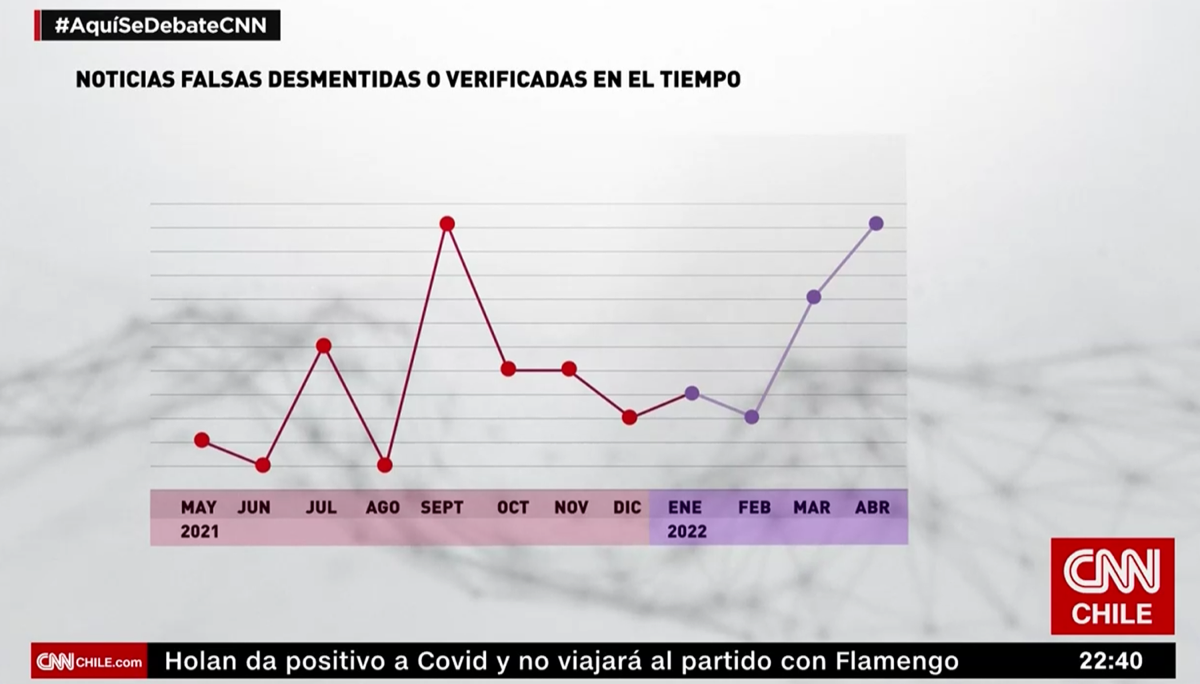
\includegraphics[width=0.32\linewidth]{imagenes/nf_en_tiempo_plesbicito_opt.png}}
    \hfill
    \fcolorbox{uclight}{white}{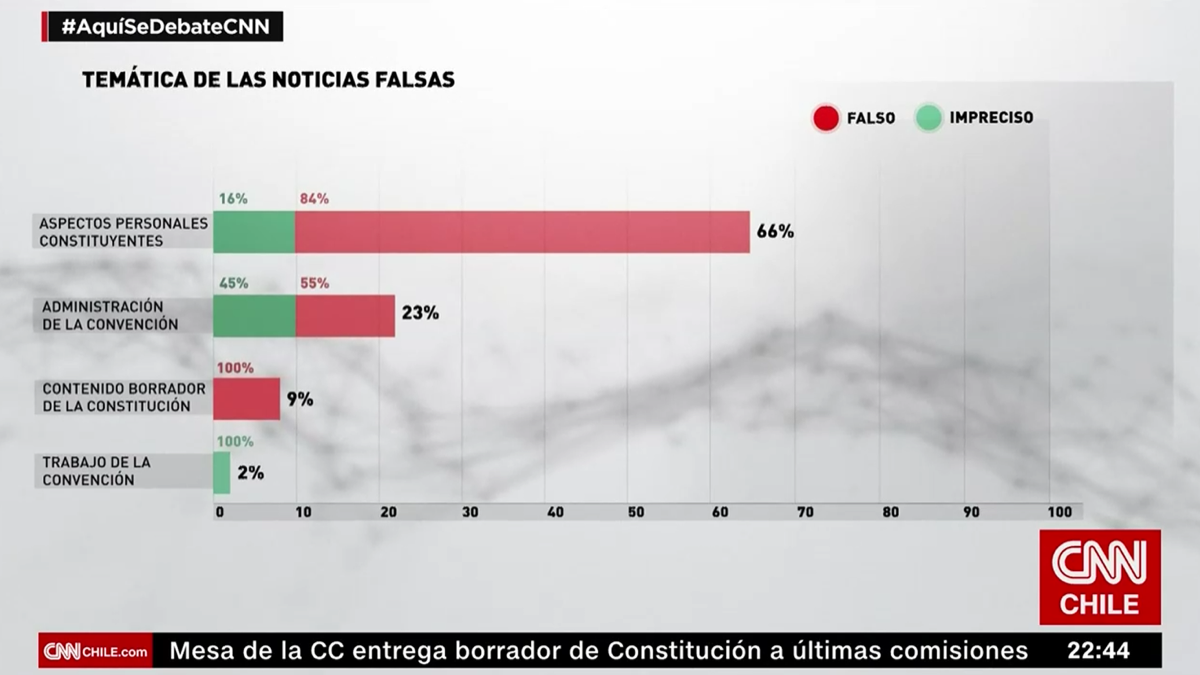
\includegraphics[width=0.32\linewidth]{imagenes/tematicas_nf_plesbicito_opt.png}}
    
    {\fontsize{12}{15}\selectfont \textit{Fuente: Plataforma Telar (M. Salda\~na, PUC)}}
\end{center}

\vspace{0.2cm}

\subsection*{\textcolor{ucred}{\textbf{2024-2025: Red de Bots AFP}}}
\begin{center}
\begin{tikzpicture}[node distance=1.0cm, auto, >=stealth, thick, scale=0.72, transform shape]
    \node[draw, rectangle, fill=ucblue, text=white, font=\bfseries, drop shadow] (afp) {ASOCIACIÓN AFP};
    \node[draw, rectangle, fill=uclight, below=of afp, align=center] (ciudadanos) {Ciudadanos en Acción\\(Bernardo Fontaine)};
    \node[draw, rectangle, fill=ucred, text=white, below left=of ciudadanos, xshift=-0.5cm] (bots) {BOTS/TROLLS};
    \node[draw, rectangle, fill=ucred, text=white, below right=of ciudadanos, xshift=0.5cm] (influ) {INFLUENCERS};
    \node[draw, ellipse, fill=darktext, text=white, below=of ciudadanos, yshift=-1.5cm, drop shadow] (fake) {DESINFORMACIÓN};

    \draw[->, line width=2pt] (afp) -- node[right, font=\small] {Financiamiento Secreto} (ciudadanos);
    \draw[->, line width=2pt] (ciudadanos) -- (bots);
    \draw[->, line width=2pt] (ciudadanos) -- (influ);
    \draw[->, line width=2pt] (bots) -- (fake);
    \draw[->, line width=2pt] (influ) -- (fake);

    % Source
    \node[below=0.2cm of fake, font=\scriptsize\itshape, text=gray] {Fuente: Investigación CIPER / Denuncia G. Winter};
\end{tikzpicture}
\end{center}

\subsection*{\textbf{\textcolor{darktext}{La Estrategia del Miedo (4 Pilares)}}}
{\fontsize{20}{24}\selectfont
Herramienta narrativa para paralizar o movilizar mediante pánico:
\begin{enumerate}
    \setlength{\itemsep}{0.15cm}
    \item \textbf{Ahorros}: Miedo a pérdida de fondos propios.
    \item \textbf{Vivienda}: Miedo a expropiación.
    \item \textbf{Salud}: Miedo al colapso del sistema.
    \item \textbf{Educación}: Miedo a desaparición de escuelas.
\end{enumerate}
}
{\fontsize{20}{24}\selectfont
\textbf{Arquitectura:} Financiamiento opaco de AFP triangulado vía agencia Artool para proteger el modelo.

\textbf{Operación:} Liderada por Bernardo Fontaine (Comando Kast) para atacar reformas y candidatas (Matthei/Jara).

\textbf{Táctica:} ``Infantería digital'' automatizada para instalar narrativas de miedo (expropiación) y desprestigio personal.
}

\end{sectionbox}

% (La sección de referencias reducida aparece a continuación)
\begin{sectionbox}{ucgreen}{REFERENCIAS}
{\fontsize{12}{14}\selectfont
    \begin{center}
        \begin{minipage}{0.24\linewidth}\centering
            \begin{minipage}[c]{0.86\linewidth}\centering
                
\includegraphics[width=0.9\linewidth]{imagenes/frame.png}
            \end{minipage}\hfill
            \begin{minipage}[c]{0.18\linewidth}\centering
                {\fontsize{10}{12}\selectfont \textbf{LINKS EN NOTION}}
            \end{minipage}
        \end{minipage}
        \hfill
        \begin{minipage}{0.24\linewidth}\centering
            \begin{minipage}[c]{0.86\linewidth}\centering
                
\includegraphics[width=0.9\linewidth]{imagenes/frame2.png}
            \end{minipage}\hfill
            \begin{minipage}[c]{0.18\linewidth}\centering
                {\fontsize{10}{12}\selectfont \textbf{PROYECTO EN GITHUB}}
            \end{minipage}
        \end{minipage}
    \end{center}
}
\end{sectionbox}
% Forzar inicio de la siguiente sección en la columna central (columna 2)
\columnbreak

% ============================================================
% COLUMNA 2
% ============================================================

\begin{sectionbox}{ucblue}{DESINFORMACIÓN DOCUMENTADA}

\subsection*{\textbf{\textcolor{darktext}{Categorización (Desórdenes Informativos)}}}
{\fontsize{20}{24}\selectfont
\begin{itemize}
    \setlength{\itemsep}{0.15cm}
    \item \textbf{Desinformación}: Contenido falso creado deliberadamente con malicia.
    \item \textbf{Malinformación}: Información real usada fuera de contexto para dañar.
    \item \textbf{Misinformación}: Falsedades compartidas sin malicia (error).
\end{itemize}
}

\vspace{0.2cm}

\subsection*{\textbf{\textcolor{darktext}{WhatsApp: Arena Cerrada (Plataforma Telar)}}}
{\fontsize{20}{24}\selectfont
\begin{itemize}
    \setlength{\itemsep}{0.15cm}
    \item \textbf{25\%} de mensajes en grupos políticos = desinformación
    \item \textbf{100\%} de fake news sobre Convención = pro-rechazo
    \item \textbf{0\%} desinformación pro-apruebo (asimetría total)
    \item Caja negra cerrada: regulación imposible
\end{itemize}
}

\end{sectionbox}
\begin{sectionbox}{ucblue}{ACTORES CLAVE}

{\fontsize{20}{24}\selectfont
\textbf{\textcolor{ucred}{\ensuremath{\blacksquare}}} \textbf{Asimetría}: Usuarios ignoran algoritmos; actores políticos + AFP coordinan

\textbf{\textcolor{ucred}{\ensuremath{\blacksquare}}} \textbf{Poder Concentrado}: Meta, X, TikTok; grupos financieros transnacionales

\textbf{\textcolor{ucred}{\ensuremath{\blacksquare}}} \textbf{Opacidad Total}: Caja negra, sin auditoría independiente, financiamiento clandestino

\vspace{0.2cm}
\begin{center}
\textbf{\textcolor{ucblue}{Control Corporativo Transnacional}}
\vspace{0.2cm}

\begin{tikzpicture}[
    edge from parent/.style={draw, -latex, thick}, 
    level 1/.style={sibling distance=5cm, level distance=3cm},
    every node/.style={draw, rectangle, rounded corners, align=center, font=\fontsize{18}{22}\selectfont, fill=uclight, drop shadow}
]
    \node[fill=ucblue, text=white, font=\fontsize{20}{24}\selectfont\bfseries] {AFP CHILENAS}
        child { node {Plan Vital\\\textbf{Generali (IT)}} }
        child { node {Provida\\\textbf{MetLife (US)}} }
        child { node {Habitat\\\textbf{Prudential (US)}} }
        child { node {Cuprum\\\textbf{Principal (US)}} };
\end{tikzpicture}
\end{center}

\vspace{0.4cm}
\textbf{\textcolor{ucblue}{Inversión en Influencia (Ene-Sep 2025)}}
\begin{itemize}
    \item \textbf{Publicidad Directa:} \$10.400 millones total. Principalmente en RRSS (\$2.225M) y Prensa Digital (\$1.890M).
    \item \textbf{Mayores Gastos:} AFP Capital (\$2.005M) y Modelo (\$1.865M).
    \item \textbf{Financiamiento Político Indirecto:} \$3.428 millones transferidos a Asoc. AFP para campañas contra reformas (no auditables).
\end{itemize}
}

\end{sectionbox}

\begin{sectionbox}{ucgreen}{RIESGOS ÉTICOS}

{\fontsize{20}{24}\selectfont
\begin{itemize}
    \setlength{\itemsep}{0.15cm}
    \item \textcolor{ucred}{\textbf{Erosión democrática}}: Sin consenso en hechos; cada ciudadano = burbuja propia
    \item \textcolor{ucred}{\textbf{Polarización subjetiva}}: Imaginamos al otro extremista. Realidad: 73\% creen derecha prohibe aborto vs. 40\% real
    \item \textcolor{ucred}{\textbf{Manipulación de género}}: 76\% ataques a mujeres candidatas, periodistas
    \item \textcolor{ucred}{\textbf{Radicalización gradual}}: Bots transforman burbuja en realidad percibida
\end{itemize}
}

\vspace{0.2cm}
{\fontsize{20}{24}\selectfont
\textbf{\textcolor{darktext}{Sesgo de Confirmación}}: La desinformación no crea miedos nuevos, sino que \textbf{amplifica ansiedades existentes} para racionalizar creencias previas.
}

\end{sectionbox}
\begin{sectionbox}{ucgreen}{PROPUESTAS VIABLES}

{\fontsize{20}{24}\selectfont
\begin{enumerate}
    \setlength{\itemsep}{0.15cm}
    \item \textbf{Transparencia algorítmica}: Auditorías externas + derecho a saber por qué ves cada contenido
    \item \textbf{Estrategia de Inoculación (Pre-bunking)}:
    \begin{center}
    \begin{tikzpicture}[node distance=1cm, auto, >=stealth, scale=1.1, transform shape]
        \node[draw, rectangle, rounded corners, fill=uclight, align=center] (exp) {1. Advertencia\\(Exposición Debilitada)};
        \node[draw, rectangle, rounded corners, fill=uclight, right=of exp, align=center] (comp) {2. Refutación\\(Comprensión)};
        \node[draw, rectangle, rounded corners, fill=ucgreen, text=white, right=of comp, align=center] (res) {3. Inmunidad\\(Resistencia)};
        \draw[->, thick] (exp) -- (comp);
        \draw[->, thick] (comp) -- (res);

        % Source
        \node[below=0.2cm of comp, font=\scriptsize\itshape, text=gray] {Fuente: UCR / Psicología Social};
    \end{tikzpicture}
    \end{center}
    \item \textbf{Diseño ético}: Veracidad sobre engagement
    \item \textbf{Regulación (UE DSA)}: Multas 10\% facturación; Brasil: removición proactiva; Chile: 11 leyes dormidas
    \item \textbf{Red fact-checking}: 40+ medios (AFP, Mala Espina) unidos contra desinformación electoral
\end{enumerate}
}

\end{sectionbox}

\end{multicols}

\vspace{0.5cm}
\begin{center}
\begin{tikzpicture}
\node [
    draw=ucblue,
    line width=3pt,
    fill=uclight,
    rounded corners=20pt,
    drop shadow={opacity=0.3,shadow xshift=5pt,shadow yshift=-5pt},
    inner sep=20pt,
    text width=0.9\textwidth,
    align=center
] (box) {
    {\fontsize{28}{34}\selectfont \textbf{\textcolor{ucblue}{REFLEXIÓN FINAL}}}\\[0.5cm]
    {\fontsize{24}{30}\selectfont \textcolor{darktext}{``Existe un consenso social amplio sobre el peligro de la desinformación, pero una inacción legislativa preocupante. Esto sugiere que la polarización es funcional a ciertos sectores políticos, quienes prefieren mantener el status quo desregulado para usar estas armas digitales en su beneficio electoral.''}}
};
\end{tikzpicture}
\end{center}

\end{document}
